% vim: textwidth=80
\documentclass{article}

% packages
\usepackage[pdftex]{graphicx}
\usepackage{listings}
\usepackage{float}

% set the code to wrap and have box
\lstset{
    frame=single,
    breaklines=true
}

% set the graphics path
\graphicspath{ {./plots/} }

\begin{document}
\title{CS 199 BD Homework 3}
\author{Richard Lee, Raj Ramamurthy, Jay Bensal\\
  NetIDs: rlee46, rmmrthy2, bensal2}

% title
\maketitle

\section{Linear Regression}
Upon building a linear regression, we noticed that there are a lot of data
points which were missing values. In order to perform a more accurate linear
regression, we removed these values. We then performed linear regression twice;
once on this model and once after performing a  Box-Cox transformation. Our code
and impressions are documented below.

\subsection{R Code: Linear Regression}
This is the commented R code that we used to create a linear model of the
original data.

\begin{lstlisting}[language=r]
#read the CSV file
crime<-read.csv('communities.data', header=FALSE)

#remove nonpredictive variables
crime<-crime[c(-1,-2,-3,-4,-5)]
crime<-crime[sample(nrow(crime)),]

#replace all '?' with NA
crime[crime == '?'] <- NA

#only take the variables w/ all the values
drop_cols <- crime[complete.cases(crime), ]

#load Data Analysis and Graphics library
library(DAAG)

#perform multivariate linear regression
fit<-lm(V128 ~ V6+ V7+ V8+ V9+ V10+ V11+ V12+ V13+ V14+ V15+ V16+ V17+ V18+ V19+ V20+ V21+ V22+ V23+ V24+ V25+ V26+ V27+ V28+ V29+ V30+ V32+ V33+ V34+ V35+ V36+ V37+ V38+ V39+ V40+ V41+ V42+ V43+ V44+ V45+ V46+ V47+ V48+ V49+ V50+ V51+ V52+ V53+ V54+ V55+ V56+ V57+ V58+ V59+ V60+ V61+ V62+ V63+ V64+ V65+ V66+ V67+ V68+ V69+ V70+ V71+ V72+ V73+ V74+ V75+ V76+ V77+ V78+ V79+ V80+ V81+ V82+ V83+ V84+ V85+ V86+ V87+ V88+ V89+ V90+ V91+ V92+ V93+ V94+ V95+ V96+ V97+ V98+ V99+ V100+ V101+ V119+ V120+ V121+ V126, data=drop_cols)

#perform k-fold cross validation
cv.lm(df=drop_cols, fit, m=4)
\end{lstlisting}

\subsection{Linear Regression Plot}
%H flag - (put it here)
\begin{figure}[H]
\centering
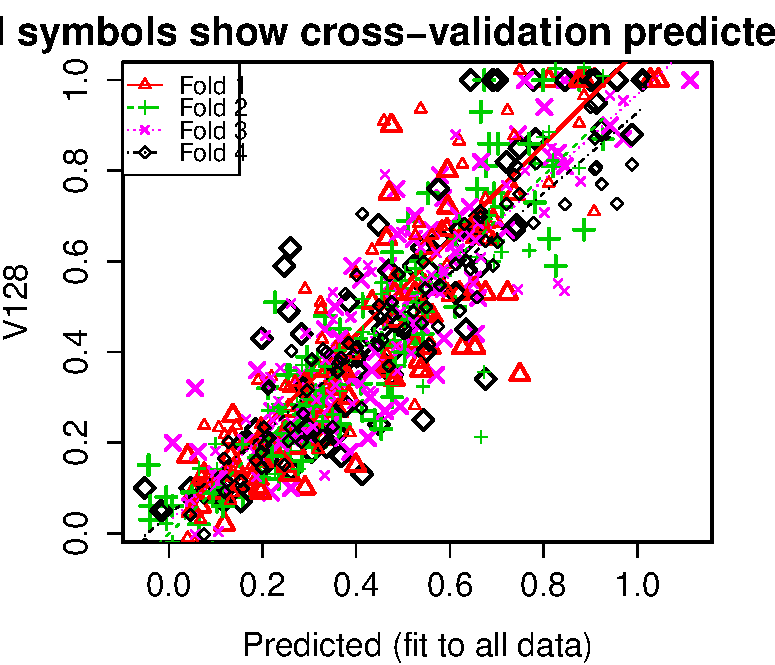
\includegraphics[width=4in]{part1a.pdf} \caption{This graph shows the
predicted fit across four different cross-validation folds of our data. Points
with a good fit are close to the line x = y. Points that are further away from
the line were predicted poorly.}
\end{figure}

Though this graph does a reasonable job of predicting fit, there are also
several problematic datapoints which you can see at the top right of the plot.
Of the two thousand original data points, only three-hundred and nineteen were
complete. It's possible that the low number of data points had an impact on the
accuracy of our results because the model built wasn't as robust as it could've
been. The metrics for four different folds are shown below.\\

\noindent
\begin{tabular}{l c r}
  Sum of squares = 3.78 & Mean square = 0.05 & n = 79\\ 
  Sum of squares = 2.30 & Mean square = 0.03 & n = 80\\
  Sum of squares = 3.48 & Mean square = 0.04 & n = 80\\ 
  Sum of squares = 3.86 & Mean square = 0.05 & n = 80\\ 
\end{tabular}\\

\noindent
\textbf{Overall:} 0.0421 ms \\
\textbf{Mean squared error:} 4.21\%.

\subsection{R Code: Box-Cox Transformation}
Here is the code we used to pick our lambda value.

\begin{lstlisting}[language=r]
#load in MASS library
library('MASS')
#pick a lambda value based on Box-Cox
boxcox(fit, lambda = seq(0, 1, 1/10), plotit=TRUE)
\end{lstlisting}

\subsection{Box-Cox plot}
%H flag - (put it here)
\begin{figure}[H]
\centering
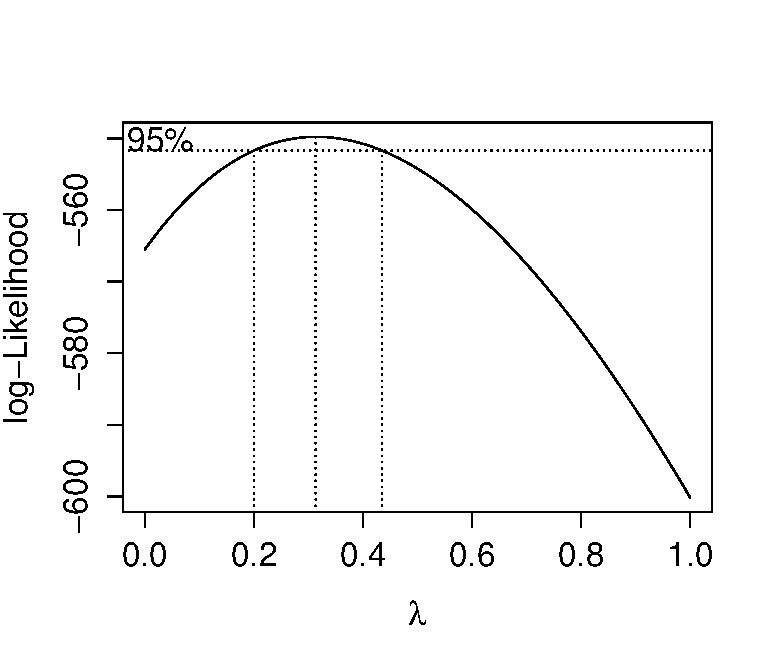
\includegraphics[width=3.8in]{boxcox.pdf}
\caption{We picked a value of l = 0.3 based on this Box-Cox graph.}
\end{figure}

\subsection{Applying the Box-Cox Transformation}
The code below transforms our data, performs a new linear regression, and then
performs k-fold cross validation with the new linear model. 

\begin{lstlisting}[language=r]
crime_lambda1 = drop_cols

#apply the Box-Cox transformation to the data
for (i in 1:nrow(crime_lambda1)){
  crime_lambda1[i, ncol(crime_lambda1)] = (crime_lambda1[i, ncol(crime_lambda1)]^0.3-1)/0.3
}

#perform multivariate linear regression based on new data
fit2<-lm(V128 ~ V6+ V7+ V8+ V9+ V10+ V11+ V12+ V13+ V14+ V15+ V16+ V17+ V18+ V19+ V20+ V21+ V22+ V23+ V24+ V25+ V26+ V27+ V28+ V29+ V30+ V32+ V33+ V34+ V35+ V36+ V37+ V38+ V39+ V40+ V41+ V42+ V43+ V44+ V45+ V46+ V47+ V48+ V49+ V50+ V51+ V52+ V53+ V54+ V55+ V56+ V57+ V58+ V59+ V60+ V61+ V62+ V63+ V64+ V65+ V66+ V67+ V68+ V69+ V70+ V71+ V72+ V73+ V74+ V75+ V76+ V77+ V78+ V79+ V80+ V81+ V82+ V83+ V84+ V85+ V86+ V87+ V88+ V89+ V90+ V91+ V92+ V93+ V94+ V95+ V96+ V97+ V98+ V99+ V100+ V101+ V119+ V120+ V121+ V126, data=crime_lambda1)

#perform k-fold cross validation on the new model
cv.lm(df=crime_lambda1, fit2, m=4)
\end{lstlisting}

\subsection{Predicted fit after Box-Cox transformation}
%H flag - (put it here)
\begin{figure}[H]
\centering
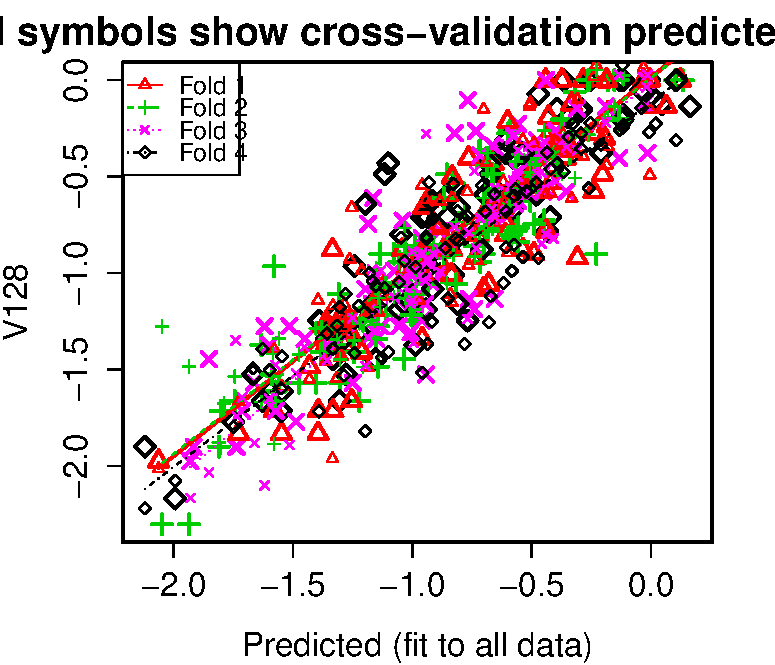
\includegraphics[width=4in]{part1b.pdf}
\caption{This graph shows the predicted fit across four different
cross-validation folds of our data after performing the Box-Cox transformation.
Points with a good fit are close to the line x = y. Points that are further away
from the line were predicted poorly.}
\end{figure}

At first glance, applying the Box-Cox transformation seems to have paid off. The
data points in this graph seem much closer to the line of best fit. In addition,
this model seems to have improved when predicting the most problematic data
points for the previous model. It's possible that having a lower number of data
points affected the Box-Cox transformation more than it effected the
untransformed data. The metrics for four different folds are shown below.\\ 

\noindent
\begin{tabular}{l c r}
  Sum of squares = 11.8 & Mean square = 0.15 & n = 79\\
  Sum of squares = 9.22 & Mean square = 0.12 & n = 80\\ 
  Sum of squares = 11.2 & Mean square = 0.14 & n = 80\\ 
  Sum of squares = 12.8 & Mean square = 0.16 & n = 80\\ 
\end{tabular}\\

\noindent
\textbf{Overall:} 0.141 ms \\
\textbf{Mean squared error:} 14.1\%.

\section{KNN}
Similar to when we performed a linear regression above, in order to perform a
more accurate linear regression, we removed the data points with incomplete
values. We then performed a k-nearest neighbors regression. Our code and
impressions are documented below.

\begin{lstlisting}[language=r]
comm<-read.csv('communities.data', header=FALSE);

#delete the first 5 vars which are not predictive
comm<-comm[c(-1,-2,-3,-4,-5)] 

#load FNN library
library('FNN')

#replace all '?' with NA
comm[comm == '?'] <- NA

#then only take the ones w/ all the values
full <- comm[complete.cases(comm),]
lapply(full, as.numeric)

full = subset(full, select=-c(V31, V102, V103, V104, V105, V106, V107, V108, V109, V111, V110, V112, V113, V114, V115, V116, V117, V118, V122, V123, V124, V125, V127))
comm_full = subset(comm, select=-c(V31, V102, V103, V104, V105, V106, V107, V108, V109, V111, V110, V112, V113, V114, V115, V116, V117, V118, V122, V123, V124, V125, V127))

#Perform nearest neighbor search with 21 neighbors
wtrain <- full[1:100,1:(ncol(full)-1)]
wtrl <- full[1:100,(ncol(full))]
wtest <- full[101:200, 1:(ncol(full)-1)]
wtel <- full[101:200, ncol(full)]
results = knn(wtrain, wtest, wtrl, k = 21, algorithm="cover_tree")

plot(as.numeric(results), as.numeric(wtel))
\end{lstlisting}

\subsection{KNN Graph}
%H flag - (put it here)
\begin{figure}[H]
\centering
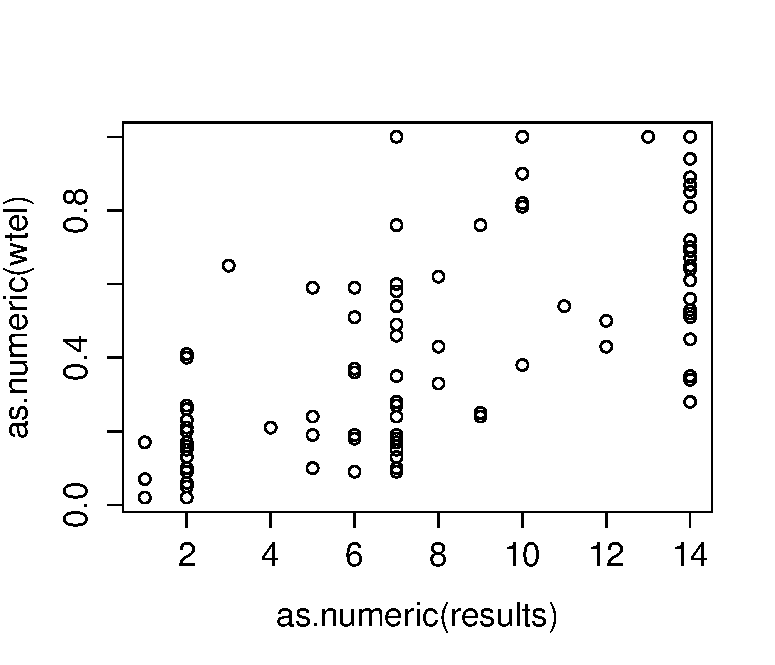
\includegraphics[width=4in]{knn.pdf}
\caption{Scatter plot of KNN results}
\end{figure}

\section{Impute}
In this section, we imputed the data and performed linear regression. Our code,
results, and impressions are below. 

\begin{lstlisting}[language=r]
#load impute library
library(impute)
#impute the data
imputed=impute.knn(as.matrix(comm_full), k=10)

#perform multivariate linear regression
fit<-lm(V128 ~ V6+ V7+ V8+ V9+ V10+ V11+ V12+ V13+ V14+ V15+ V16+ V17+ V18+ V19+ V20+ V21+ V22+ V23+ V24+ V25+ V26+ V27+ V28+ V29+ V30+ V32+ V33+ V34+ V35+ V36+ V37+ V38+ V39+ V40+ V41+ V42+ V43+ V44+ V45+ V46+ V47+ V48+ V49+ V50+ V51+ V52+ V53+ V54+ V55+ V56+ V57+ V58+ V59+ V60+ V61+ V62+ V63+ V64+ V65+ V66+ V67+ V68+ V69+ V70+ V71+ V72+ V73+ V74+ V75+ V76+ V77+ V78+ V79+ V80+ V81+ V82+ V83+ V84+ V85+ V86+ V87+ V88+ V89+ V90+ V91+ V92+ V93+ V94+ V95+ V96+ V97+ V98+ V99+ V100+ V101+ V119+ V120+ V121+ V126, data=as.data.frame(imputed$data))

#perform k-fold cross validation
cv.lm(df=as.data.frame(imputed$data), fit, m=4)
\end{lstlisting}

From looking at this graph, we can conclude that the classifier is not very
good with KNN. If this classifier was good, we would see a trend closer to a line
with slope of roughly 1/10.

\subsection{Impute plot}
%H flag - (put it here)
\begin{figure}[H]
\centering
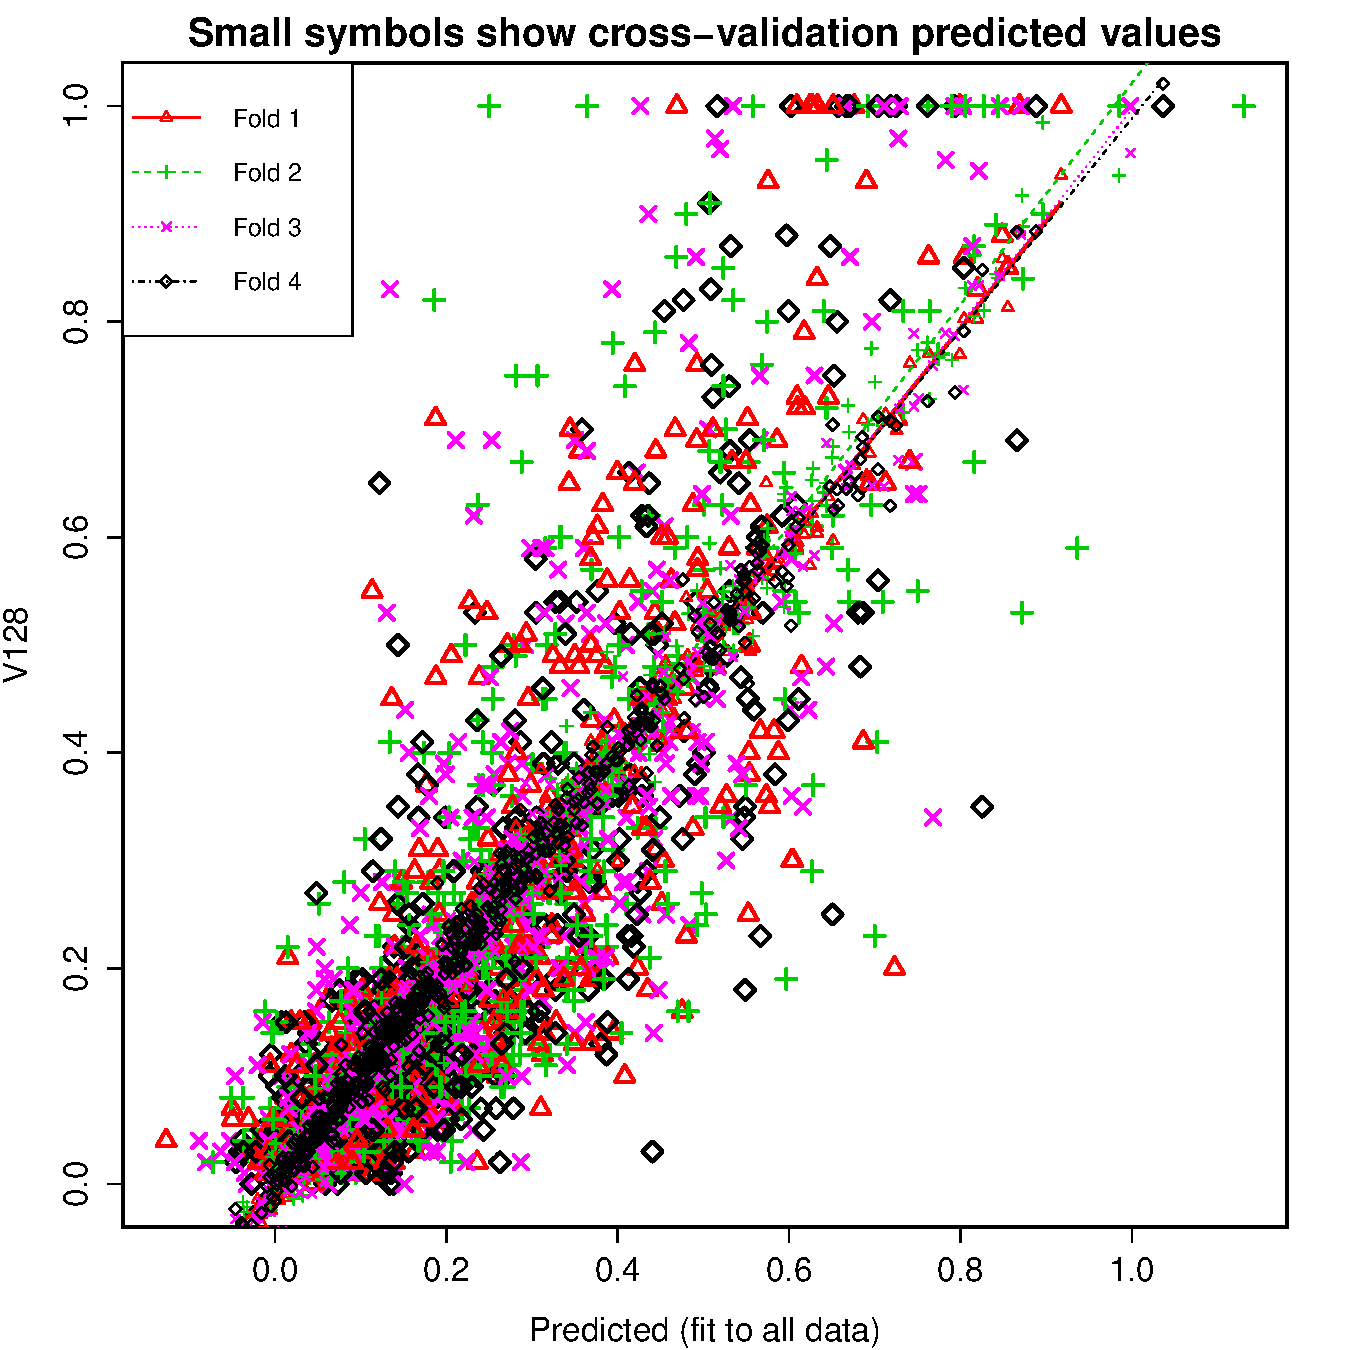
\includegraphics[width=4in]{impute.pdf}
\caption{This graph shows the predicted fit across four different
cross-validation folds of our imputed data. Points with a good fit are close to
the line x = y. Points that are further away from the line were predicted
poorly.}
\end{figure}

The linear model based off of the imputed data provided the highest accuracy of
the linear models that we built. One possible reason for this could be the high
number of data points. Though every data points wasn't as complete as could be,
the sheer number of data points used to build the model helped improve accuracy.
The metrics for four different folds are shown below.\\

\noindent
\begin{tabular}{l c r}
  Sum of squares = 8.69 & Mean square = 0.02 & n = 498\\ 
  Sum of squares = 10.8 & Mean square = 0.02 & n = 499\\ 
  Sum of squares = 9.43 & Mean square = 0.02 & n = 499\\ 
  Sum of squares = 8.83 & Mean square = 0.02 & n = 498\\ 
\end{tabular}\\

\noindent
\textbf{Overall:} 0.0189 ms \\
\textbf{Mean squared error:} 1.89\%.

\section{Modified Nearest Neighbor Search}
\end{document}
